\section{Removing Mutable Storage}

Now that we can freely retrieve immutable structures, we can focus on other
storage variables. A challenge we faced is that the protocol of NIPoPoWs
dependents on $DAG$ structure which is a mutable hashmap. This logic is
intuitive and efficient to implement in most traditional programming languages
such as C++, JAVA, Python, JavaScript, etc. However, as our analysis
demonstrates, such an algorithm cannot be efficiently implemented in Solidity.
This is not due to the lack of support of look-up structures, but because
Solidity hashmaps can only be contained in storage. Other
mutable structures, such as $ancestors$ that are stored in the persistent
memory also affect performance, especially for large proofs.

We make a keen observation regarding the possible position of the \emph{block
of interest} in the proof which lead us the constriction of an architecture
that does not require $DAG$, $ancestors$ or any other complementary structures.
We will use the notation from~\cite{nipopows} to present our claim.

\noindent \textbf{Position of block of interest.} NIPoPoWs are sets of sampled
interlinked blocks, which means that they can be perceived as chains. If
$\pi_1$ differs from $\pi_2$, then a fork is created at the index of the last
common ancestor ($lca$). The block of interest, $b$, lies at a certain index
within $\pi_{subm}$ and indicates a stable predicate~\cite{nipopows,
generic-client} that is true for $\pi_{subm}$. The case in which $b$ is absent
from $\pi_{subm}$ is aimless, because the submission automatically fails since
the predicated is evaluated against $\pi_{subm}$. We will refer to such aimless
actions as \emph{irrational} and components that are included in such actions
irrational components, i.e.  irrational proof, blocks etc. We will use the term
\emph{rational} to describe non-irrational actions and components.

The entity that initiates the contest of $\pi_{subm}$, tries to prove the
falseness of the underlying predicate against $\pi_{cont}$. This means that, if
the block of interest is included in $\pi_{cont}$, then the contest is
irrational.

In the NIPoPoW protocol, proofs' segments $\pi_{subm}\{:lca\}$ and
$\pi_{cont}\{:lca\}$ are merged to prevent adversaries from skipping or adding
blocks, and the predicate is evaluated against $\pi_{subm}\{:lca\} \cup
\pi_{cont}\{:lca\}$. We observe that $\pi_{submit}\{:lca\}$ can be omitted
because there is no block \{$B : B \notin \pi_{subm}\{:lca\} \land B \in
\pi_{cont}\{:lca\}$\} that results to positive evaluation of the predicate.
This is due to the fact that $b$ is not included in $\pi_{cont}\{:lca\}$, and,
presumably there is no $B$ such that $b = B$.

\begin{figure}[h]
    \begin{center}
        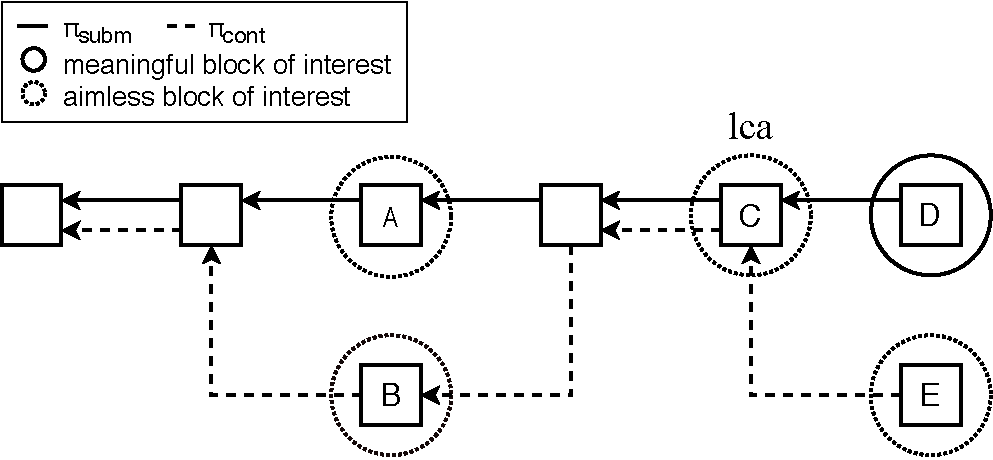
\includegraphics[width=1\columnwidth]{figures/boi-position.pdf}
    \end{center}
    \caption{Fork of two chains. Solid lines connection blocks of $\pi_{subm}$
    and dashed lines connect blocks of $\pi_{cont}$. Given the configuration,
    blocks in dashed circles are irrational blocks of interest, and the block i
    in the solid circle is a rational block of interest.}
    \label{fig:boi-position}
\end{figure}

In Figure~\ref{fig:boi-position} we display a fork of two proofs. Solid lines
connect blocks of $\pi_{subm}$ and dashed lines connect blocks of $\pi_{cont}$.
Examining which scenarios are rational depending on different positions of the
block of interest, we observe that blocks \texttt{B}, \texttt{C} and \texttt{E}
do not qualify, because they are included only in $\pi_{cont}$. Block
\texttt{A} is included in $\pi_{subm}\{:lca\}$, which means that $\pi_{cont}$
is an irrational contest. Given this configuration, the only rational block of
interest is \texttt{D}.

\newcommand{\pis}{\pi_{subm}}
\newcommand{\pic}{\pi_{cont}}
\newcommand{\pitr}{\pi_{cont}^{tr}}

\noindent \textbf{Minimal forks.} By combining the above observations, we
derive that, $\pi_{cont}$ can be truncated into $\pi_{cont}\{:lca\}$ without
affecting the correctness of the protocol. We will term this truncated proof
$\pitr$ \footnote{We cannot proceed to further truncation of $\pitr$, because
    in the NIPoPoW protocol blocks within segment $\pi\{:lca\}$ of each proof
are required for the score calculation.}. Security is preserved if we require
$\pitr$ to be a \emph{minimal fork} of $\pis$. A minimal fork is a fork chain
that shares exactly one common block with the main chain. Proof $\tilde\pi$,
which is a minimal fork of proof $\pi$, has the following attributes:

\begin{enumerate}
\item $\pi\{lca\} = \tilde\pi[0]$
\item $\pi\{lca:\} \cap \tilde\pi[1:] = \O$
\end{enumerate}

By requiring that $\pitr$ is a minimal fork of $\pis$, we prevent an adversary
from dispatching an augmented $\pitr$ to claim better score against $\pis$.
Such an attempt is displayed in Figure~\ref{fig:adversary-minimal-fork}.

\begin{figure}[h]
    \begin{center}
        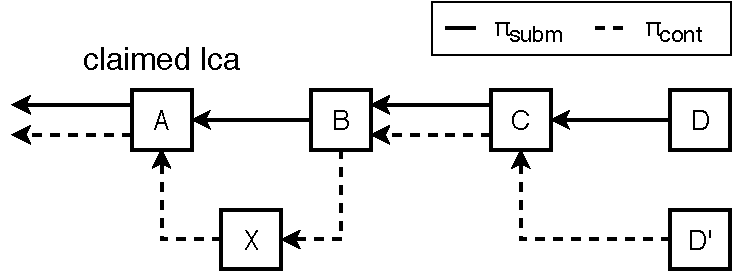
\includegraphics[width=0.78\columnwidth]{figures/adversary-minimal-fork.pdf}
    \end{center}

    \caption{An adversary tries to send a malformed proof consisting of blocks
    \{A, X, B, C, D'\} that achieves better score against \{A, B, C, D\}. This
    attempt is rejected due to the minimal-fork requirement.}

    \label{fig:adversary-minimal-fork}
\end{figure}

In Algorithm~\ref{algo:minimal-fork}, we show how minimal fork technique is
incorporated in our client, replacing $DAG$ and $ancestors$. In
Figure~\ref{fig:minimal-fork} we show how the performance of the client has
improved.

\renewcommand{\genesis}{\textsf{G}}

\begin{algorithm}

    \label{alg:minimal-fork}
    \caption{The \textsf{NIPoPoW} client using the minimal fork technique}

    \begin{algorithmic}[1]

    \Contract{crosschain}
    \State $\textsf{events} \gets \bot;$ $\genesis \gets \bot$
    \Function{\sf initialize}{$\genesis_{remote}$}
        \State \genesis $\gets \genesis_{remote}$
    \EndFunction
    \Function{\sf submit}{$\pis$, $e$}
        \State \textsf{require}($\pis$[0] = $\genesis$)
        \State \textsf{require}($\textsf{events$[e]$} = \bot$)
        \State \textsf{require}($\textsf{valid-interlink}(\pis)$)
        \State \textsf{events$[e]$.hash} $\gets$ \textsf{H}($\pis$)
        \State \textsf{events$[e]$.pred} $\gets$
        \textsf{evaluate-predicate}(\textsf{$\pis$}, $e$)
    \EndFunction
    \Function{\sf contest}{$\pisa$, $\pitr$, $e$, $f$}
        \Comment{$f$: fork index}
        \State \textsf{require}($\pitr$[0] = $\pisa[f]$)
        \Comment{check fork head}
        \State \textsf{require}(\textsf{events}$[e]$ $\ne$ $\bot$)
        \State \textsf{require}(\textsf{events$[e]$.hash} $=$ \textsf{H}($\pisa$))
        \State \textsf{require}(\textsf{valid-interlink}($\pitr$))
        \State \textsf{require}(\textsf{minimal-fork}($\pisa$,
        $\pitr$, $f$))
        \State \textsf{require}(\textsf{score}($\pitr$)
            $>$ \textsf{score}($\pisa[f:]$))
        \State \textsf{events$[e]$.pred} $\gets$
            \textsf{evaluate-predicate}($\pitr$, $e$)
    \EndFunction
    \Function{\sf minimal-fork}{$\pi_1$, $\pi_2$, $f$}
        \For{$p\ in\ \pi_1$}
            \If{$p \in \pi_2$}
                \State\Return false
            \EndIf
        \EndFor
    \EndFunction
    \EndContract
    \vskip8pt
    \end{algorithmic}
\end{algorithm}



\begin{figure}[h]
    \begin{center}
        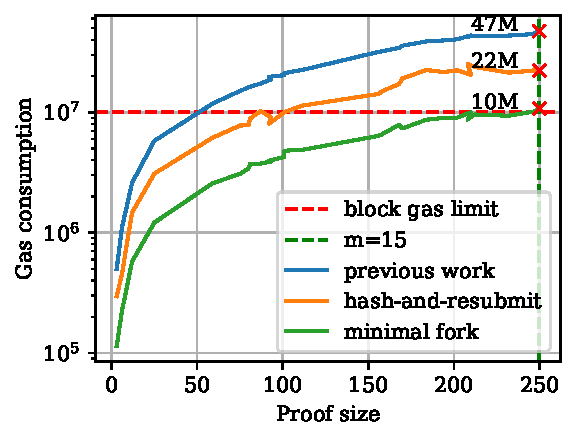
\includegraphics[width=1\columnwidth]{figures/minimal-fork.pdf}
    \end{center}
    \caption{}
    \label{fig:minimal-fork}
\end{figure}
